\documentclass[10pt,twocolumn,letterpaper]{article}

\usepackage{statcourse}
\usepackage{times}
\usepackage{epsfig}
\usepackage{graphicx}
\usepackage{amsmath}
\usepackage{amssymb}

% Include other packages here, before hyperref.

% If you comment hyperref and then uncomment it, you should delete
% egpaper.aux before re-running latex.  (Or just hit 'q' on the first latex
% run, let it finish, and you should be clear).
\usepackage[breaklinks=true,bookmarks=false]{hyperref}


\statcoursefinalcopy


\setcounter{page}{1}
\begin{document}


%%%%%%%%%%%%%%%%%%%%%%%%%%%%%%%%%%%%%%%%%%%%%%%%%%%%%%%%%%%%%%%
% DO NOT EDIT ANYTHING ABOVE THIS LINE
% EXCEPT IF YOU LIKE TO USE ADDITIONAL PACKAGES
%%%%%%%%%%%%%%%%%%%%%%%%%%%%%%%%%%%%%%%%%%%%%%%%%%%%%%%%%%%%%%%



%%%%%%%%% TITLE
\title{\ Time Series Forecasting on Energy Consumption \\
  \large ML Project Final Report. Hertie School, 2022}

\author{Kabir Sandrolini\\
{\tt\small k.sandrolini@mds.hertie-school.org}
\and
Katalin Bayer\\
{\tt\small k.bayer@hertie-school.org}
\and
Jiayu Yang\\
{\tt\small 213444@hertie-school.org}
\and
Angela Duarte Pardo\\
{\tt\small a.duarte-pardo@hertie-school.org}
}

\maketitle
%\thispagestyle{empty}



% MAIN ARTICLE GOES BELOW
%%%%%%%%%%%%%%%%%%%%%%%%%%%%%%%%%%%%%%%%%%%%%%%%%%%%%%%%%%%%%%%


%%%%%%%%% ABSTRACT
\begin{abstract}
 
 Machine Learning has developed into a key tool for modeling energy consumption. Accurate forecasts improve the performance of electric systems by reducing the amount of production surpluses and energy shortages. Well-constructed ML models of energy consumption can therefore prevent energy blackouts and reduce wasteful overproduction, cutting costs (for producers, consumers, and states in general) and contributing towards a more sustainable future. Our aim in this project is to evaluate the performance of different supervised Machine Learning algorithms (ARIMA, Extra Trees, Gradient Boosting and Support Vector Machines) and an Auto Machine Learning Framework (AutoGluon) in predicting power consumption for the city of Tetouan, Morocco based on time-series data from 2017. The data set includes different markers of the weather conditions during that time, such as temperature, wind speed, and humidity. We build on work from an existing study, with a different approach in terms of data cleaning/transformation and models selected. We use a variety of models in an attempt to find which one best optimizes both accuracy and computational efficiency.
   
 In our exploration, we used ARIMA linear regressions as our baseline. With our more advanced models, we found that while SVM performs very poorly on the task, ExtraTrees and Gradient Boosting models performed pretty well. This paper provides important insight on how to optimally predict energy consumption based on climatic data, indicating which models are most accurate and efficient. The results have important revenue and sustainability implications for businesses, policymakers, governments, and society at large.
\end{abstract}




%%%%%%%%% BODY TEXT
%%%%%%%%% INTRODUCTION
\section{Introduction}

Accurately forecasting consumption levels has important implications for society in terms of energy policy and sustainability. Accurate energy consumption models can reduce the risk of energy shortages (i.e. blackouts), ensuring that communities are not left without electricity, which can lead to critical economic and infrastructural issues for societies. Conversely, reducing energy consumption, in particular energy waste, is an essential element for mitigating climate change. Accurate forecasts would also help utility companies avoid overproduction and subsequent energy waste (as it is difficult to store surplus energy), saving money and natural resources. The economic benefits would be significant, as producers would be able to cut costs and in theory pass on these savings to consumers. Policymakers, governments, and energy-focused NGO's could use the findings from the model to understand which factors most influence energy consumption (e.g. season, temperature, humidity, etc), which will be crucial in the face of climate change, COVID-19, geopolitical tensions, and socioeconomic fluctuations. The findings from such a model could also support a transition to a more sustainable energy grid. This is why much attention has been devoted to the improvement of electric systems' forecasting \cite{kalimoldayev2020analysis}. These models are providing increasingly accurate predictions of how consumption values fluctuate as a function of variable weather conditions and temporal factors \cite{salam2018comparison}. 

While this project has clear practical policy motivations, it is equally stimulating from a technical perspective, as we will be working with a rich data set. In this project\footnote{Here is the link to our GitHub repository \url{https://github.com/zeitgeist-hash/GRAD-C24-Machine-Learning.git}} we evaluate the performance of five different machine learning models -- ARIMA, Gradient Boosting, ExtraTrees, Support Vector Machines (SVM), and Auto ML framework AutoGluon developed by Amazon -- for predicting energy consumption in Tetouan, Morocco during 2017. We will use data on weather conditions as well as temporal variables as predictors. We use Python to train and test our models, compare our results to a baseline ARIMA model, and discuss their differences in performance. 


%%%%%%%%% RELATED WORK
\section{Related Work}

The data has previously been used in a study published by two professors at Abdelmalek Essaadi University in Morocco, indicating that it is high-quality reliable data, and providing us a useful baseline with which to compare our findings. The paper ``Comparison of Machine Learning Algorithms for the Power Consumption Prediction: Case Study of Tetouan city''\cite{salam2018comparison} finds that hour and temperature are the most important predictive features, and that the random forest model consistently achieved the best results in terms of accuracy. 

Similarly, the exploration of Sejin Yang\cite{githubNYC} uses the correlation of energy usage and weather data to predict future electric energy consumption in New York City buildings using Long-Short Term Networks. Their exploration shows that interest in energy consumption is not only limited to academia, but also impacts the private sector and those interested in mitigating climate change. 

This brief exploration of related work showcases two important aspects. First,  the prediction of electric energy consumption based on weather conditions is gaining more and more attention in the scientific community concerned with climate change. Second, In choosing between various modelling options, we must optimize between accuracy (error measurement) and computational efficiency. We hope to be able to contribute to the field and to the research on climate change mitigation in a broader sense by evaluating a unique selection of Machine Learning approaches.

%%%%%%%%% PROPOSED METHOD
\section{Proposed Method}

By design, we chose not use the same models or follow the same approach as the original study. The authors of that study predict energy consumption at both 10 minutes and 1 hour intervals, generating three different models per zone of the city. We instead average the 10-minute readings into a single hourly observation, and the mean of the three zones into a single composite geographic average, as for our purposes we did not need such a granular approach to the data. More importantly, the previous paper does not explicitly account for the time-series nature of the data. Instead, since the data is not IID, we will adjust for its temporal nature by using an ARIMA model as a baseline and differencing the target variable to make the data stationary. Moreover, we focus on supervised learning models (ExtraTrees, SVM and Gradient Boosting) and AutoGluon. With this approach, we expect to better account for the time dependency of our data, so that we get a better sense of ML's performance in time series forecasting problems.

We developed all of our models in Python, primarily using the pmdarima, sk-learn, and Autogluon packages. 

\subsection{Baseline - ARIMA model}

The key variable of interest, mean power consumption in Tetouan, has been recorded periodically in 10-minute increments - which we have aggregated into hourly increments. This, by definition, constitutes time series data. When confronted with model estimation the structure of the data, left untreated, creates issues in traditional estimation approaches. This is because time series data do not satisfy the $i.i.d$ assumptions, as the underlying data generating process is not a stochastic process. If the time series component is not stationary, regular estimation processes lead to problems with correlated error terms and biased coefficients due to trending data over time, for example.

Accounting for  time series data is typically done by using either ARIMA or VAR type models. In this project we only consider ARIMA type models; VARs only include Auto Regressive (AR) lags, which yields less parsimonious results and can generally be computed quickly using OLS or GLS. However, we have motivated this decision due to the additional seasonal daily lags (24-hour increments) that are captured by the Moving Average (MA) lags, which the ARIMA models use. Here the underlying estimation process is maximum likelihood estimation and indeed, this drastically increases the computational runtime. Ultimately, our results show that amongst the class of ARIMA models, the optimal time series model is a Seasonal Auto Regressive Integrated Moving Average eXogenous (SARIMAX) model. This subclass of ARIMA includes seasonality lags as well as differencing the time series first observations, as opposed to ARIMA which only considers AR and MA lags. Our final optimal model has the following structural form:

\begin{align*}
SARIMAX(2, 1, 0)\times(1, 0, [1, 2], 24)\\
y_t^* = c + \phi_1 y_{t-1}^* + \phi_2 y_{t-2}^* + \phi_3 y_{t-24}^* + \phi_4\epsilon_{t-24}\\ 
+ \phi_5\epsilon_{t-48} + \epsilon_t
\end{align*}

The primary tool to carry out the analysis was the pmdarima package. The details of the key procedures are discussed in the Baseline Model Experimental Details section.

\subsection{Machine Learning Models Architecture}

Our data set includes labels for Mean Power Consumption. We therefore used supervised learning models for our prediction task: Extra trees, Gradient Boosting, Support Vector Machines, as well as an AutoML framework  -- AutoGluon.
\begin{itemize}
  
\item\textit{Extra Trees} or \textit{Extremely Randomized Trees} are an improvement of Decision Trees. Like Random Forests, Extra Trees combine the predictions of many trees into a single prediction, by choosing the best split between the subsets of features. Unlike Random Forests, Extra Trees randomize both attributes and cut-points in the node splitting process (thus reducing variance and execution time), and uses the whole data set for the training process (reducing bias)\cite{geurts2006extremely}. Thus, they end up having similar performance to Random Forests, but through a simpler algorithm.\cite{ExtraVsRandom}

\item\textit{Support Vector Machines} are versatile Machine Learning models that work well for both linear and non-linear classification and regression tasks. Learning tasks performed with SVM are characterized by the algorithm finding the largest possible margin between hyperplanes that define "classes" of instances on a given space. SVM Regression (or SVR) models use these margins to fit as many possible instances, while limiting violations\cite{geron2019hands}. To do this, SVR maps the input data $ x\in R^{n}$ into a high-dimensional feature space through a non-linear mapping $\phi$ and then approximates the function, given by
$$f(x)=w^{T}\varphi(x_{i})+b$$
where \textit{w} is the weight vector and \textit{b} is the bias. SVR treats this function as an optimization problem. This means that it wants to find the narrowest tube around the surface that minimizes the prediction error $\frac{1}{2}w^{t}w$ subject to $\mid y_{i}-w^{T}(x_{i})-b\mid\leq\varepsilon$. Here $\varepsilon $ is user set highest possible deviation from the target variables $ y\in\Re $.\cite{amirkhalili2020comparison}


\item\textit{Gradient Boosting} is an algorithm that boosts weak learners into strong learners. It has relatively fast training times, as well as high performance. Unlike the Bagging and Stacking methods, the Boosting training process is a tandem approach where the weak learners are trained sequentially, with each weak learner learning from the previous one and eventually combining the predictions of all the learners to produce the final prediction. For this model we used Scikit-Learn's $GradientBoostingRegressor$ class.

\item\textit{AutoGluon} is an open-source AutoML framework  that enables easy-to-use and easy-to-extend machine learning approaches developed by Amazon \cite{ge2020analysis}. It only needs a few lines of simple and elegant code to ensemble multiple models, leveraging automatic hyperparameter tuning and stacking them in multiple layers for comparison. AutoGluon enables users to utilize state-of-the-art techniques without expert knowledge and conduct significant gains in accuracy and time-efficiency \cite{AutoGluon-Tabular2020}.

\end{itemize}

%%%%%%%%% EXPERIMENTS
\section{Experiments}

This section provides details of our data and the experiments we performed to optimize our predictions of the average power consumption in Tetouan based on weather and temporal factors.

\subsection{Data}
The data set was retrieved from the University of California, School of Information and Computer Science’s online Machine Learning repository\cite{DataSet}. It is originally derived from a study conducted by faculty at the Abdelmalek Essaadi University in Morocco in 2018. The raw data was sourced "from the SCADA system of the regional distribution company of drinking water and electricity (AMENDIS)" \cite{salam2018comparison}. The data contains energy consumption observations for 3 districts in Tetouan \cite{salam2018comparison}. It is a comprehensive data set with no missing values, and has a multivariate time series structure: each attribute is observed in 10-minute increments, over a 1-year time period from January 1 2017 to December 30 2017. The power consumption of Tetouan is divided into three source stations: Quods, Smir and Boussafou. Each data point represents the aggregated power consumption in each respective station or zone. The data set is therefore labelled. 

Moreover, for each power consumption observation, the data set includes weather-related observations that have also been recorded in 10-minute intervals. These include temperature, humidity, wind speed, general diffuse flows, and diffuse flows \cite{salam2018comparison}. Power consumption is measured in kilowatt-hours and temperature is measured in celsius. Since the data contains seasonal and hourly trends, it required some cleaning and wrangling before it can be used in time series models. 

\begin{figure}[h!]
\centering
\centerline{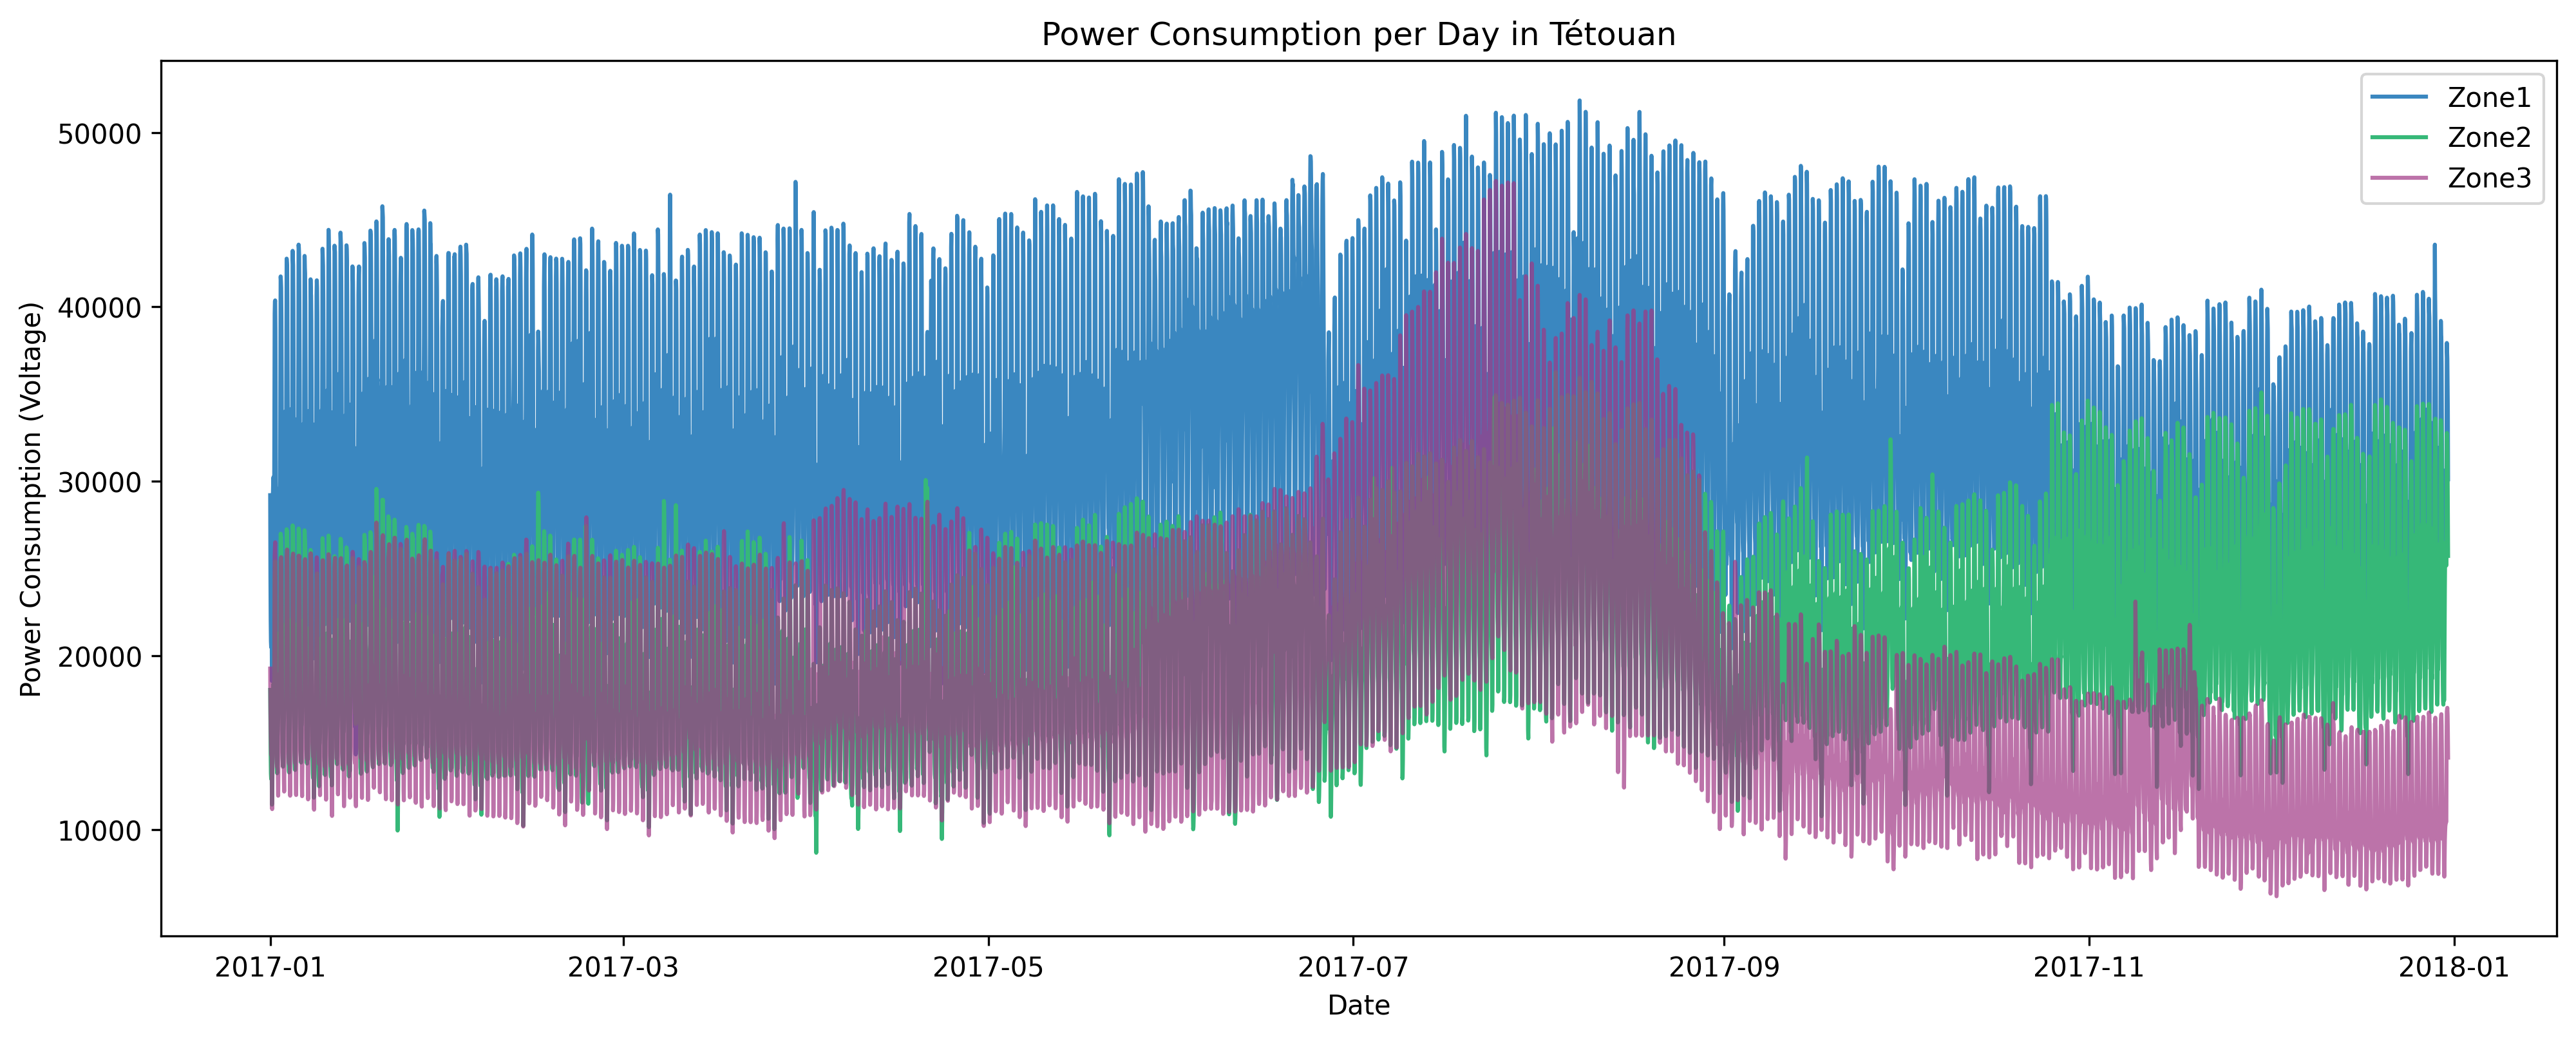
\includegraphics[width=8.5cm]{figures/OverallConsumption.png}}
\caption{Power consumption per 10 minutes intervals in the three source stations of Tetouan}
\label{fig}
\end{figure}

\textit{Figure 1} visualizes energy consumption for the three zones every 10 minutes over the course of a year. We can already identify some significant seasonal fluctuations in power consumption, with a notable increase during the summer in all three zones (particularly in Zone 3 - Boussafou). This makes sense: Tetouan has a Mediterranean climate with mild temperatures in the winter and high temperatures in the summer. The spike in summer consumption is likely caused by an increase of air conditioning, as well as a general increase in the population caused by the summer influx of tourists.   

We performed many transformations on the data for our analysis, extracting temporal dummy variables from the original data. Since energy consumption varies highly by time of day in addition to the season, we included variables for days, months, hours, and so on. We also computed the mean consumption of the 3 power stations so as to have one composite outcome variable (our target variable). Finally, we computed hourly readings as an average of the original 10-minute observations, scaling our number of observations down by a factor of 6. We felt that given the scope of our project, and since we are relatively less familiar with the specific dynamics of Tetouan, our study would not benefit from the same granularity as the original study (which analyzed separately by district and 10-minute intervals). Instead, our modifications should not only improve model performance and run-time, but will also help us isolate and identify larger trends in the data.


\subsection{Software and Hardware} 
We coded our project entirely in Google Colab, using our local machines to access Google's cloud servers. To implement our ML models, we relied on the following Python packages: numPy, matplotlib, pandas, SciKitLearn, PMDARIMA, and AutoGluon. 

%%%%%%%%%%%%%%%%%%%%%% EVALUATION METHOD%%%%%%%%%%%%%%%%%%%%%%%%%%%
\subsection{Evaluation methods}

Evaluating the accuracy of different machine learning models is an essential part of an ML project, as it provides common metrics for comparing and optimizing model selection. We used three main metrics: R Squared ($R^2$), Mean Squared Error (MSE) / Root Mean Squared Error (RMSE), and Mean Absolute Error (MAE). All these metrics indicate the difference between our predicted values and the actual values, and can be calculated by using different functions from scikit-learn library. 

$R^{2}$ or the \textit{coefficient of determination} provides a measure of how well we can explain the variance in the dependent variable from the variance of other predictors.

$$R^{2} =1-\frac{\sum_{i=1}(\hat{y}^{(i)}-y^{(i)})^{2}}{\sum_{i=1}^{m}(y^{(i)}-\Bar{y})^{2}}.$$

In the formula, $\hat{y}^{(i)}$ are the predicted values and $\Bar{y}$ corresponds to the mean of observed values. $R^{2}$ is an intuitive measure of error for regression problems because a measure of 1 means the model captures all variance of the dependent variable, while lower values indicate relative worse model fit. However, many advise against over-relying on this measure to test the performance of Machine Learning algorithms in time-series forecasting. The $R^{2}$ value for a time series model could seemingly indicate high accuracy, but can be caused by the auto-correlation due to time-dependency, as successive observations are intrinsically related to each other\cite{10.2307/2286421}. A high value could thus provide a misleading indication of accuracy. For this reason, we will not report $R^2$ values for our ARIMA models, and we will provide it for the other models, but it will not be our main comparative measure.

Therefore, other metrics are more widely used in machine learning to evaluate and compare such models. MSE/RMSE and MAE both measure the distance between the vector of predictions and the vector of target values.\cite{geron2019hands} Let $\mathbf{X}$ be the feature values matrix, $h$ the prediction function or hypothesis, such that $\hat{y}^{i}=h(x^{(i)})$ is the predicted value for the instance $x^{(i)}$. 

Then, MSE is calculated as: 

$$MSE(\mathbf{X}, \mathbf{h}) =\frac{1}{m}\sum_{i=1}^{m}(h(x^{(i)})-y^{(i)})^{2}.$$

And RMSE is the square root of the MSE.
MAE or \textit{Mean absolute error} is calculated as:
$$MAE(\mathbf{X}, \mathbf{h}) =\frac{1}{m}\sum_{i=1}^{m}\lvert{h(x^{(i)})-y^{(i)}}\rvert.$$

Although RMSE/MSE and MAE are cost functions, they penalize different aspects of the prediction: RMSE is more sensitive to outliers than MAE, so it is preferable in more concentrated distributions.\cite{geron2019hands}. We consider all measures to ensure a comprehensive comparison.

%%%%%%%%%%%%%%%%%%%%%% EXPERIMENTAL DETAILS%%%%%%%%%%%%%%
\subsection{Experimental details:} 

For data pre-processing, we grouped the data into 1 hour intervals and calculated the mean of all the features on that time interval. Then we calculated a composite target variable with the mean consumption value of the three zones or stations. 

After the pre-processing, we calculated the results of the \textit{Augmented Dickey Fuller} (ADFuller) test, which is a statistical test, part of the \textit{statsmodels} package, that indicates whether the times series is stationary or not. Stationarity is a key requirement for many estimation methods. In non-stationary time series the mean, variance and auto-correlation structures change over time, a clear indicator of $i.i.d$ assumptions being violated. We cannot expect unbiased estimators and good machine learning predictions, if our models violate key assumptions \cite{Stationarity}. The test has a null hypothesis: "the time series is non-stationary (i.e. it has a unit root)", which can be rejected if $p-value<0.05$ \cite{ADFTest}. We run the test for our target variable (\textit{MeanConsumption}. The results in \textit{Table 1} confirm that the time series in Tetouan is indeed non-stationary, and that this non-stationarity is due to some peaks in the consumption of the summer months (shown also in the second column of our table). As we will explain later in this section, our baseline and machine learning models use differences of observations to make the time series stationary. The results of the differentiation can also be observed in the $\Delta$Target column of \textit{Table 1}. 

\begin{table}[h]
\footnotesize
\centering
\begin{tabular}{|l|c|c|c|}
\hline
Statistic & Target & SummerMonths & $\Delta$Target\\
\hline
ADF & -2.57 &  -1.39 & -16.26 \\
\hline
p-value & 0.0985 &  0.59 & $3.54e^{-29}$ \\
\hline
\end{tabular}
\caption{Results of the Adfuller test on the target vatiable.\label{tab:some_table}}
\end{table}

\textbf{Baseline Model Experimental Details:}
In determining the baseline model, we used the pmdarima package, and primarily its auto\_arima function. This function automates all of the necessary data transformations, as carried out manually for the other models above, and then proceeds to algorithmically determine the optimal ARIMA model. The pm.utils.tsdisplay() function returns the following three visualisations. Figure \ref{figACF} below shows the desirable stationarity of our power consumption data after taking the first difference. The ACF plot indicates the strong seasonal component of the data series which informed the choice of including seasonal lags in our ARIMA model.

\begin{figure}[h]
\centering
\centerline{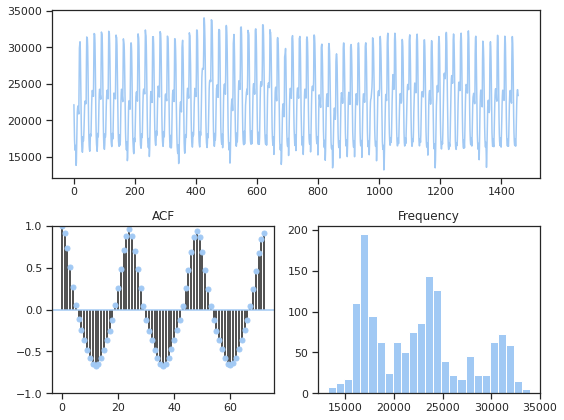
\includegraphics[width=8cm]{figures/ACF_plot.png}}
\caption{Top: Plotting the Differenced Data. Bottom Left: ACF plot. Bottom Right: Histogram.}
\label{figACF}
\end{figure}


In order to determine this optimal model, the auto\_arima function performs a step-wise procedure across various model specifications and determines the best model from four different specifications to start with. out of these four, the best model is chosen according to the lowest Akaike Information Criterion. The other models are then updated in a stepwise adjustment of the parameters with respect to current best model, AICs are recomputed and compared again and the new best model gets updated. This iterative process is repeated until no model with a lower AIC can be found and a threshold is reached. This is another feature than can be tuned by the user, among the many parameters and choices the user makes.

Additionally, a key difference in the implementation between the ARIMA baseline model and the other ML models we considered was the test-training split. In auto\_arima, which uses scikitLearn's TimeSeriesSplit, which splits the data into several sets of training and testing data whilst retaining the time series element. As the auto\_arima function runs, the training sets updates in a rolling manner until the last test set is reached. This is then used as the validation set and the model forecast on this validation set, is used as our comparison measure.

\textbf{Other Model's Experimental Details:}
As for the other machine learning models, we  split the training set, validation set and test set in a ratio of 6:2:2. Since the data is based on time-series, this separation had no random component (if we did the usual train/test splitting, we would risk having future observations predicting past observations). Our validation and testing sets correspond then to the 40\% of the newest observations so that the training is done in the earliest part of the time-series and the predictions on the subsequent observations.

\begin{figure}[h]
\centering
\centerline{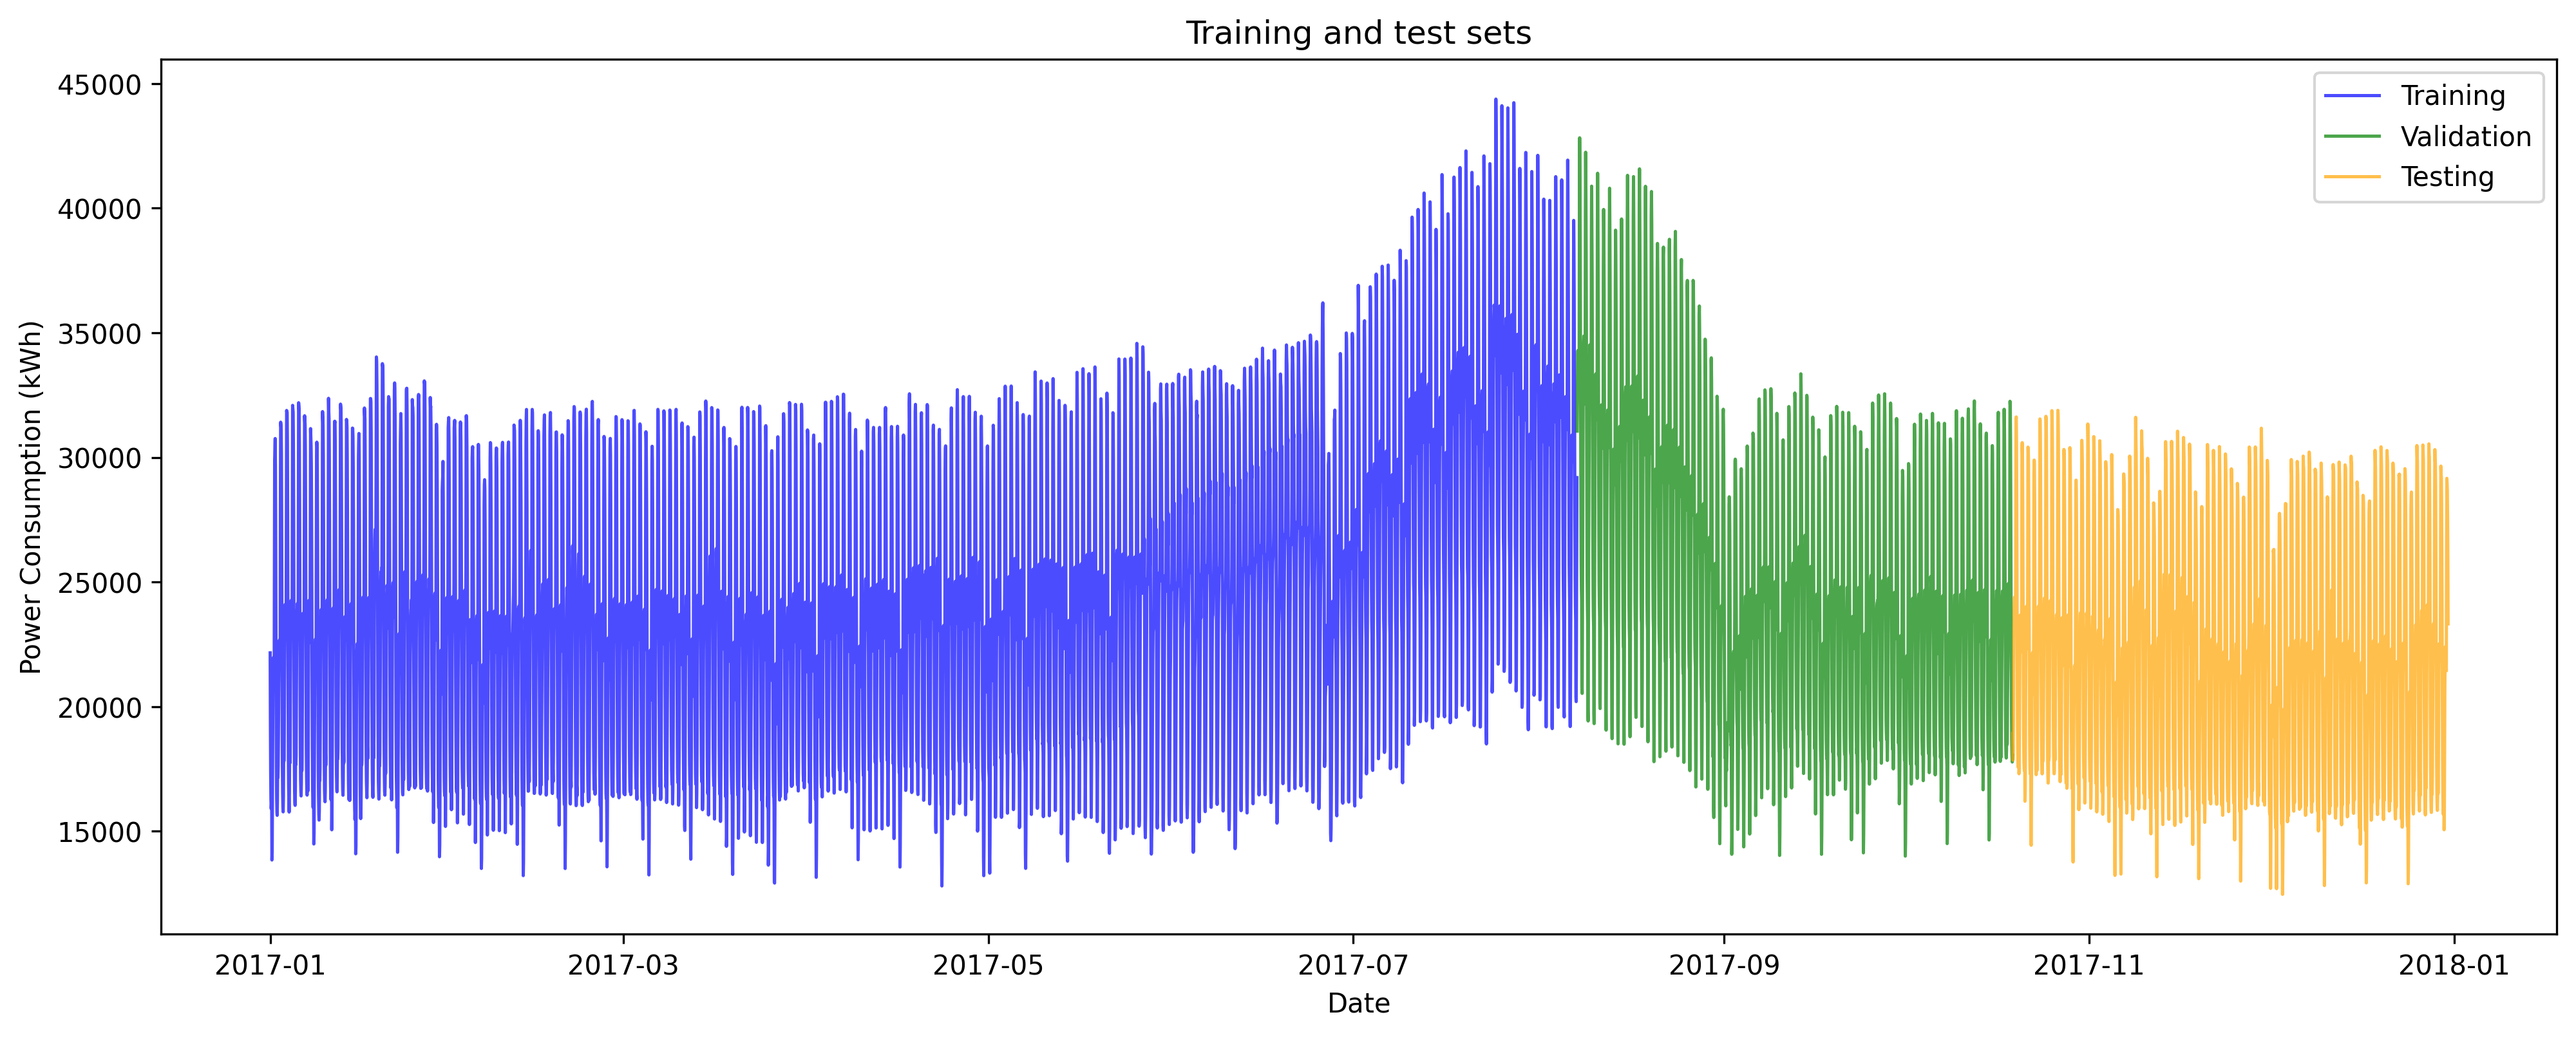
\includegraphics[width=8cm]{figures/split.png}}
\caption{Set splitting into training, validation and testing sets. \cite{browne2000cross}}
\label{fig}
\end{figure}

We then calculated the difference between the target variable at time $t$ and at time $t-1$. This differentiation allowed us to have a stationary data set, as can be seen in Table1 and Appendix 10.4\label{fig_stationary}. For better accuracy of our predictions, we added 1-hour, 2-hour and 24-hour lagged differences to the weather and seasonality covariates. These time lags are those that minimize the ARIMA model's AIC and therefore are considered the appropriate lags to include. Whilst the function also determines the relevant MA lags, it is becomes very complicated compute these manually in order to include them so we determined to exclusively include AR lags in the remainder of the ML models we test.

For SVM, ExtraTrees and Gradient Boosting models, we initially trained them with default settings and applied them on the validation sets. Then we compared their performances based on their evaluation metrics. After that we did the fine-tuning process to find best model parameters with GridSearchSV function for those models. Table 3 shows the optimal parameters that we used for our testing set prediction. However, AutoGluon could prototype classical machine learning and deep learning solutions, and find optimal hyperparameters automatically with a few lines of code.

\begin{table}[h]
\footnotesize
\centering
\begin{tabular}{|l|c|c|}
\hline
Model & Fine-tuning & Training time \\
\hline
ExtraTrees & max\_depth=11 & 2.3s\\
 & n\_estimators=20 & \\
  &  min\_split=60 & \\
\hline
 SVM & C=1000 & 2.78s \\
 & gamma= 0.0001 & \\
\hline
Gradient Boosting & max\_depth=3 & 2s\\
 & n\_estimators=60 & \\
  & min\_split=80 & \\
\hline
\end{tabular}
\caption{Model configurations after running GridSearch for parameter tuning.\label{tab:some_table}}
\end{table}

%%%%%%%%%%%%%%%%%%%%%% RESUlTS%%%%%%%%%%%%%%%%%%%%%%%%%%%
\subsection{Results} 
We calculated $R^{2}$, RMSE, MSE and MAE as our evaluation metrics for each of the models, except for the ARIMA model. Table \ref{tab:some_table} shows the accuracy and error measures for the baseline and other models we trained in the experimental phase of the project. It is worth noting that in time-series analytics a smaller RMSE indicates better results\cite{amirkhalili2020comparison}.

\begin{table}[h]
\footnotesize
\centering
\begin{tabular}{|l|c|c|c|c|}
\hline
Model & $R^{2}$ & RMSE & MSE & MAE \\
\hline
Naive & / & 1152.50  & 1328259.10 &  760.19\\
ARMA & & & & \\
\hline
Mean & / & 966.15 & 933447.24 & 669.56\\
SARIMAX & & & & \\
\hline
Composite & / & 975.38 & 951366.01 & 681.46\\
SARIMAX & & & & \\
\hline
ExtraTrees & 0.97 & 340.57 & 115990.42 & 241.32\\
\hline
 SVM & 0.09 & 1749.24 & 3059843.46 & 1246.14 \\
\hline
 GradBoosting & 0.96  & 348.45 &  121420.78 & 245.48 \\
\hline
\end{tabular}
\caption{$R^{2}$, RMSE, MSE, and MAE for the models used in the experiment.\label{tab:some_table}}
\end{table}

\paragraph{Comments on the quantitative results.} 
\begin{itemize}
\item\textbf{ARIMA} 
As soon as the auto\_arima parameters have been defined and the code is running, there is little the user can still adjust in that moment. Rather than trying to manually recompute the auto\_arima processs, we decided to let this code run three times, with different consumption aggregation methods. Firstly, the “Naïve” forecast, which predicts the mean consumption of Tetouan City purely based on the power consumption 24-hours ago, a simple AR(24) model. We chose this as our simple forecast since the data exploration highlighted the importance of the daily lag. Secondly, the “Mean” forecast, which lets auto\_arima determine the number of optimal lags across various classes of ARMA models. Finally, the last forecast has been denoted the ”Composite” forecast, first each Zone’s individual power consumption is predicted using auto\_arima, and then the total Mean Consumption is computed as the mean across the three zone’s forecast. The visualisation of only the Mean forecast (only for the forecasted time period) is plotted below in Figure \ref{fig_forecast_plot} below. The plots for the types of forecast methods can be found in the appendix in Figure \ref{fig_naiveplot} and Figure \ref{fig_compplot}. 
\begin{figure}[h]
\centering
\centerline{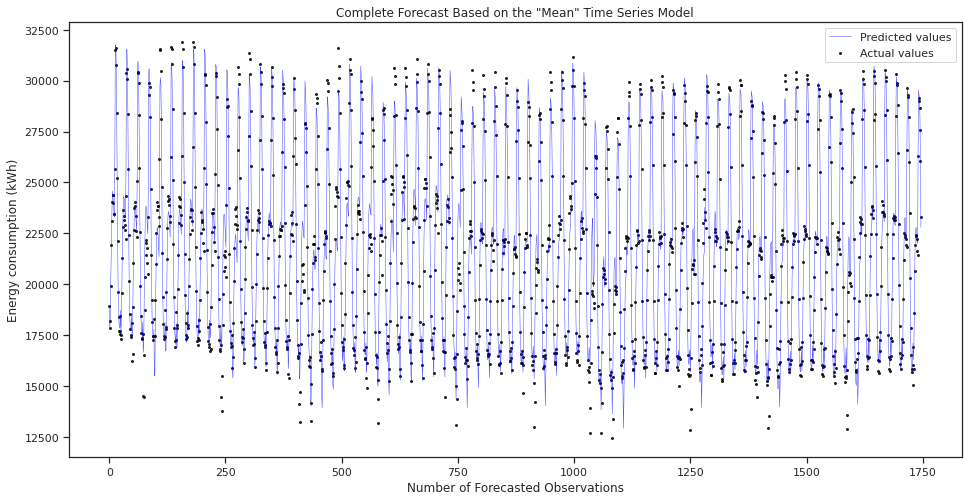
\includegraphics[width=8cm]{figures/Mean_forecast.png}}
\caption{Mean Consumption forecast only for the forecast horizon}
\label{fig_forecast_plot}
\end{figure}

\item\textbf{SVR} 
Even with the optimal configurations resulting from the grid search algorithm, our SVR model underfits the power consumption stationary time series. As the results table \ref{tab:some_table} show, the error rates that we obtained when testing the model are high (an error of almost $1750$, the RMSE, is considerable given that the differentiated means range between -5269 and 8193 KWh)). Also, as can be seen in Figure \ref{fig}, the prediction values seem to pick up the oscillation trend of the time series, but not its variation along the 'y' axis.
\begin{figure}[h]
\centering
\centerline{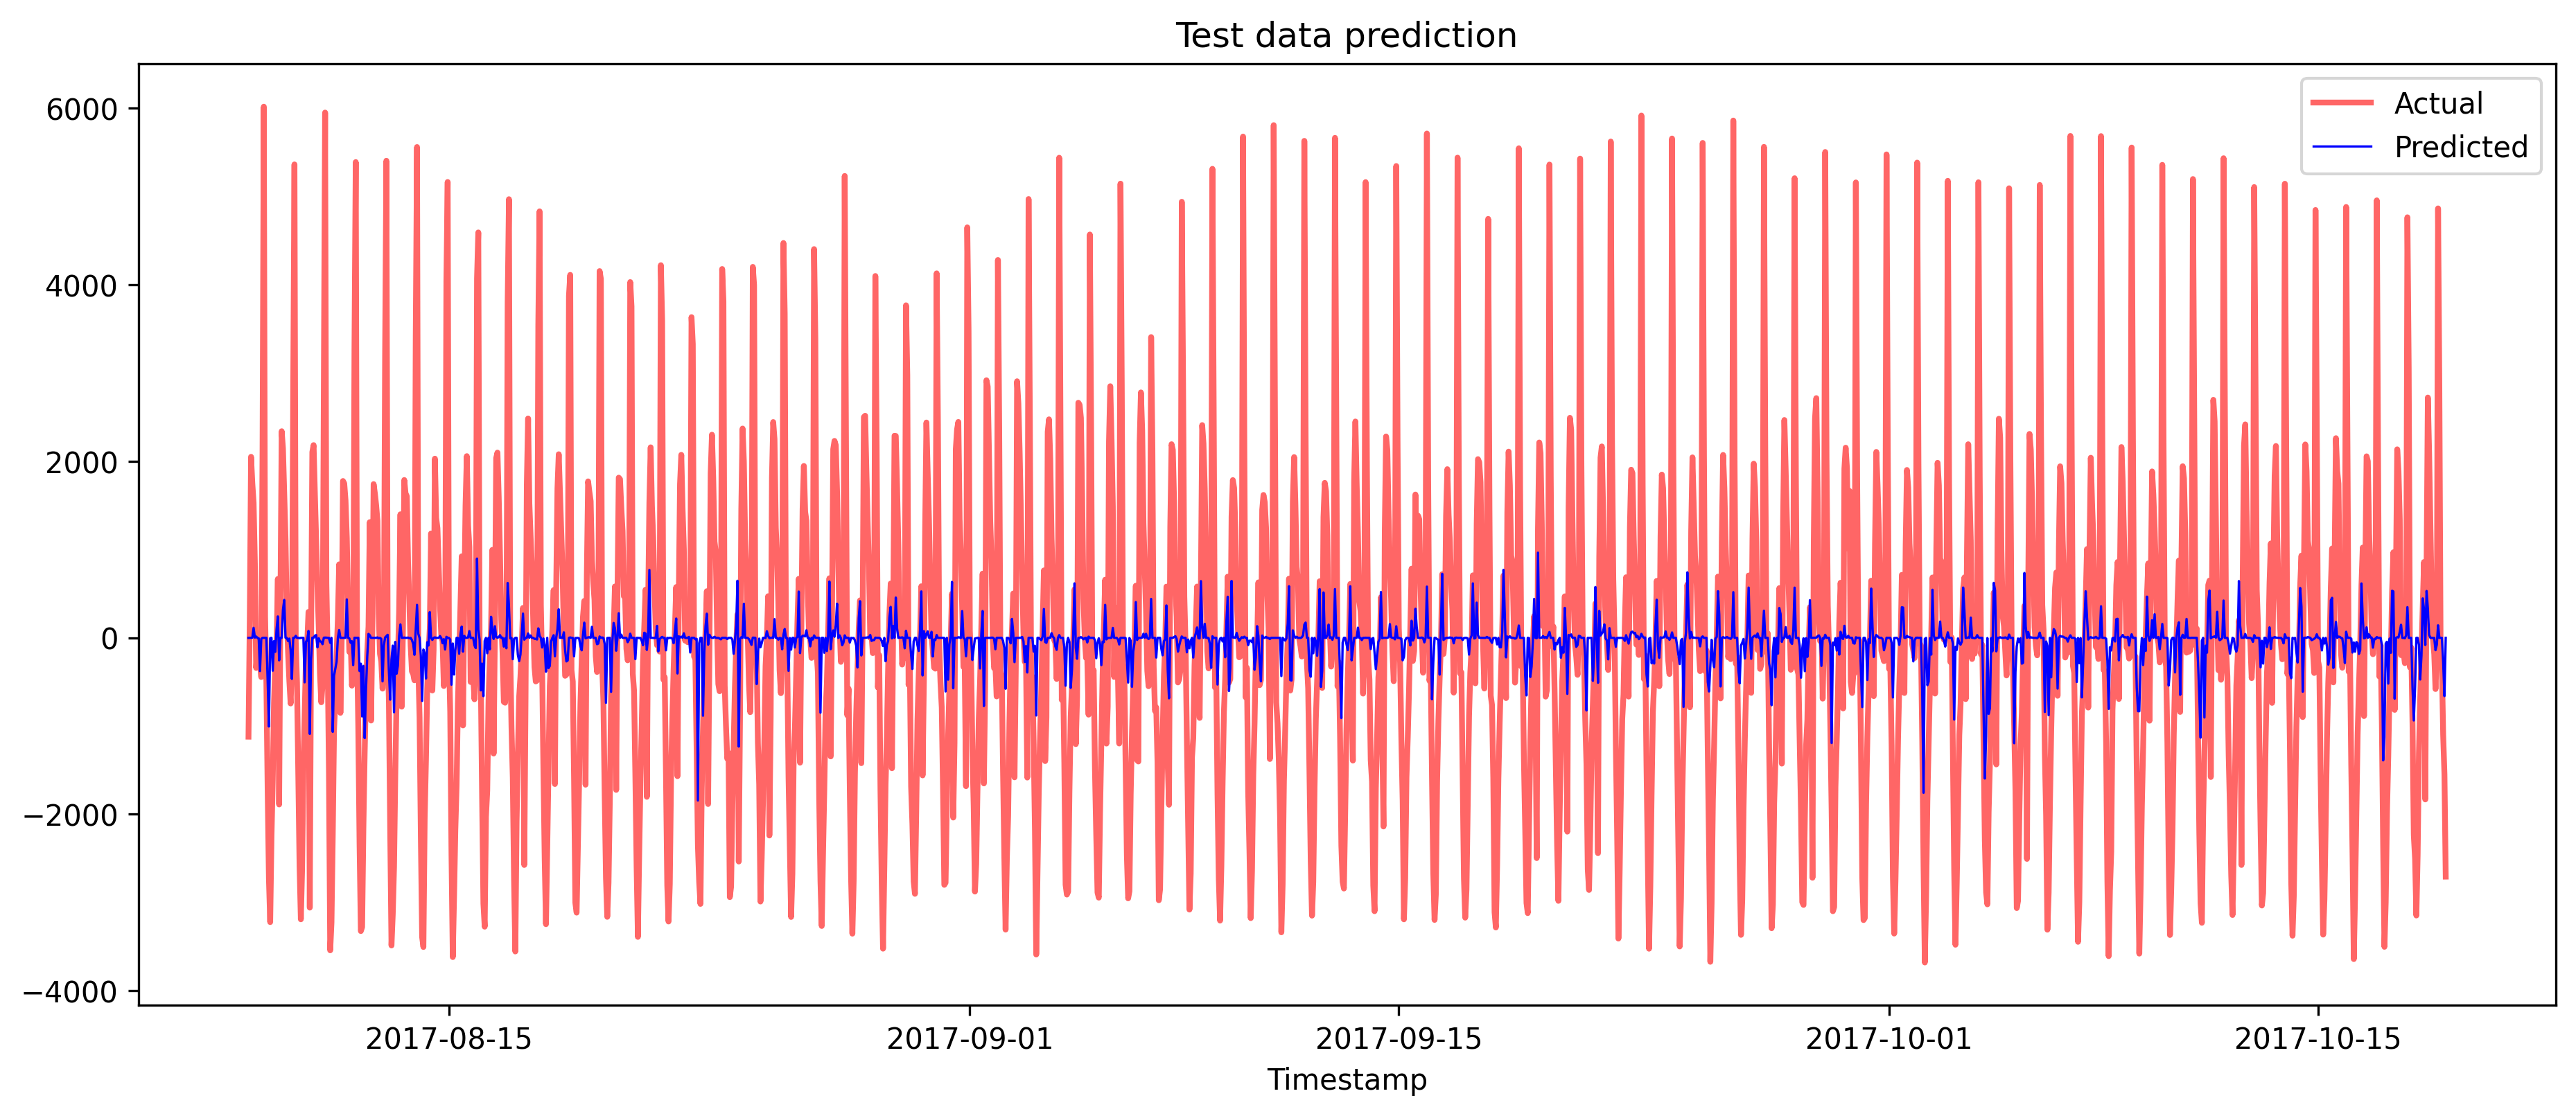
\includegraphics[width=8cm]{figures/svr_test.png}}
\caption{Predicted vs actual values of optimal SVR}
\label{fig}
\end{figure}

\item\textbf{ExtraTrees \& GradientBoosting} 
We are satisfied with the results of ExtraTrees \& Gradient Boosting that their RMSE are around 340 after fine-tuning, they performed slightly worse on the testing set than on the validation set as expected. It proves that both of them are very stable and suitable for dealing with regression problems.

\begin{figure}[h]
\centering
\centerline{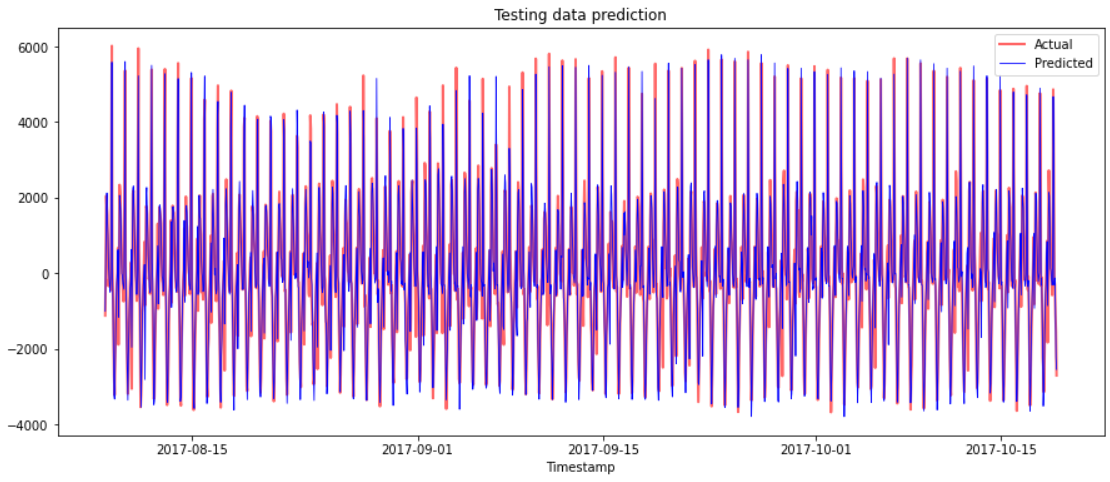
\includegraphics[width=8cm]{ET.png}}
\caption{Predicted vs actual values of optimal ExtraTrees}
\label{fig}
\end{figure}

\begin{figure}[h]
\centering
\centerline{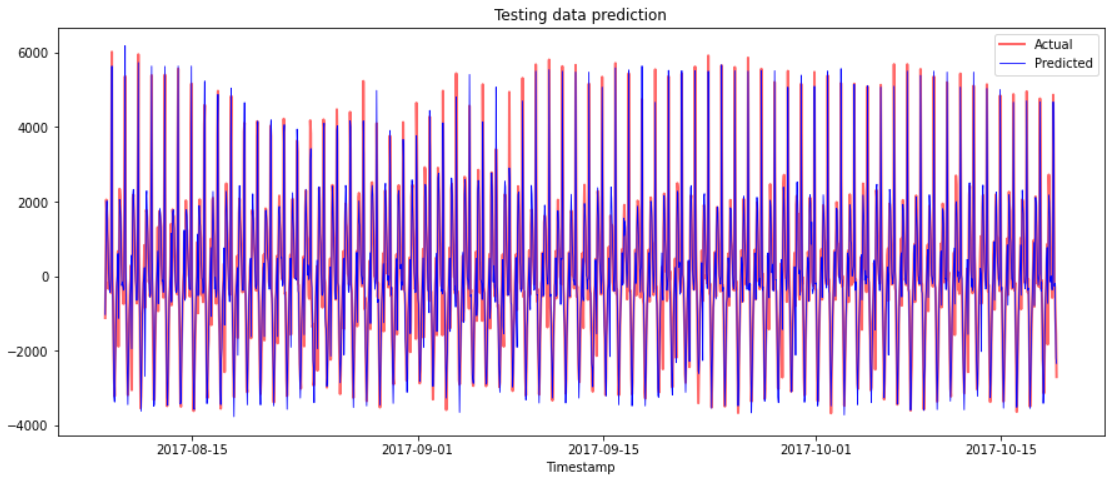
\includegraphics[width=8cm]{GB.png}}
\caption{Predicted vs actual values of optimal GradientBoosting}
\label{fig}
\end{figure}

\item\textbf{AutoGluon}
 Here we specified the particular evaluation metric (MSE) and AutoGluon could tailor its models to optimize the metric. For evaluation metrics where higher values are worse (like MSE), AutoGluon can flip their signs and print them as negative values during training (as it internally assumes higher values are better). Then we called leader-board to see the per-model performance to see more details such as MSE, training time etc. The leader-board shows 12 ML models in total and ranks these models according to how well they perform.

\begin{figure}[h]
\centering
\centerline{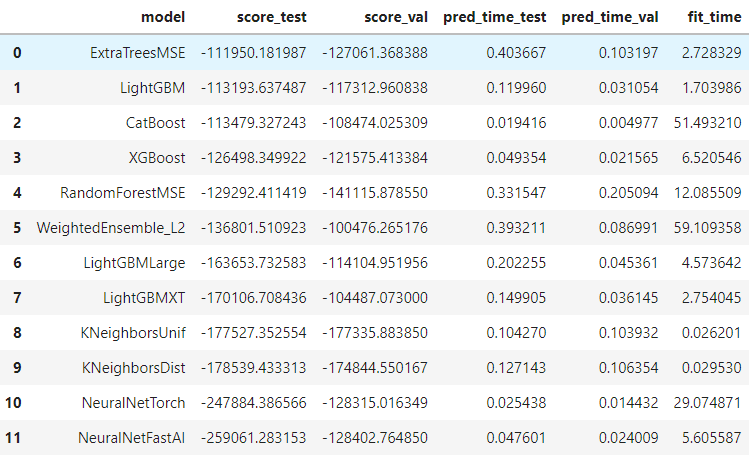
\includegraphics[width=8cm]{Auto.png}}
\caption{Leaderboard of AutoGluon}
\label{fig}
\end{figure}

\end{itemize}


%%%%%%%%% ANALYSIS
\section{Analysis}

Before evaluating the performance of our models in the time-series forecasting task, it is worth going back to the nature of the task: predicting the mean energy consumption based on weather data. The temporal dependency of the data makes it very easy for the learning algorithms to reproduce the trend of the previous data point instead of finding a function of the target based on the covariates.  This is why the $R^{2}$ score is not a very good measure of accuracy when comparing models for time-series forecasting. The success of our models is then measured by their ability to adequately minimize RMSE and to pick up the temporal trends of the data. 

Generally speaking, all three results from the regular time series models capture the variance in the dependent variable rather well - in spite of adding no further explanatory variables and purely relying on the lags, seasonality, and moving averages. The regression analysis output in the Appendix show that all of the lag terms determined by auto\_arima are statistically significant with p-values of 0. The intuition is sound too, the power consumption of today primarily depends on the power consumption an hour ago, two hours ago, and yesterday. The difference this 24-hour, seasonality lag makes is indicated by Figure \ref{fig_seasonalityplot} down below. The fact that the Naive forecast performed worst across the three models was hardly surprising, as we include more, relevant lags, the models forecasting ability improves. The expectation was that the composite forecast would outperform the mean as the model would be able to adapt to each Zone individually first. However, despite this not being the case, all performance measures we computed are very close to each other in magnitude. 

\begin{figure}[h]
\centering
\centerline{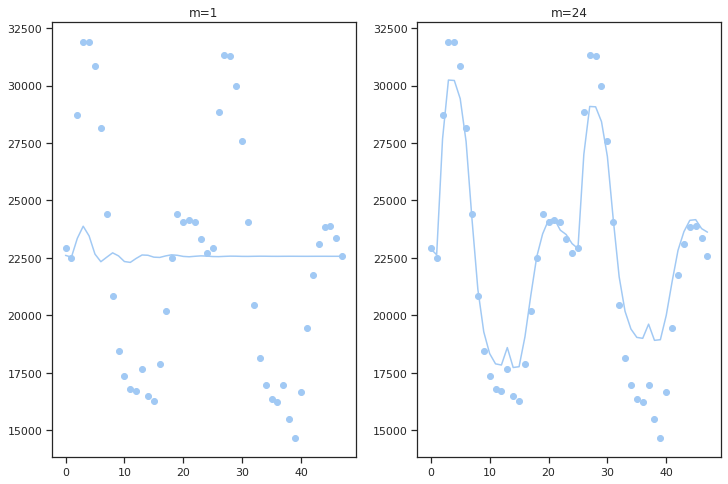
\includegraphics[width=8cm]{figures/Seasonality_plot.png}}
\caption{Search model without (m =1) vs. with (m=24) seasonality}
\label{fig_seasonalityplot}
\end{figure}


As for the SVR model, despite the optimization process through GridSearchSV, its performance was the worst of all the studied models: not only was the RMSE the highest, but the predictions didn't reach the full amplitude of the labels in our dataset. Despite our expectations, this is not so surprising. A plausible explanation might be that SVM tend to do better with scaled data\cite{amirkhalili2020comparison} (which stabilizes both the mean and variance of the data). The process we performed to make the time-series stationary, stabilized only the mean but not the variance (something we decided on not to lose the variations that we wanted to be able to predict).This might explain why our SVR model was "blind" to the high peaks of the hourly differences in power consumption. 

However, we can also see that ExtraTrees and Gradient Boosting models performed quite well on validation sets and testing sets. In terms of the characteristics of these algorithms, ExtraTrees and GradientBoosting belongs to ensemble learning that can often achieve significantly better generalisation performance than a single learner by combining multiple learners. From the results of testing sets (both of their RMSE are around 340), they are very robust even in the face of a lot of outliers and time series data.

From the leaderboard (Figure 4) of auto-ML framework AutoGluon, we found that half of the models performed as good as fine-tuned ExtraTrees and GradientBoosting models on the testing set, however the other models performed very generally. Decision trees and boosting techniques have better performance but KNeighbors techniques are not very good.

%%%%%%%%% CONCLUSIONS
\section{Conclusions}
Our main achievement is that we successfully implemented the time-series nature of our data not only into our baseline model but also included some lag elements in our standard machine learning algorithms. Arguably this is the main result of the paper as can be seen from the ARIMA models, the recurring time aspect by itself, which is reflected in the forecast plots of the baseline model. The next step was to consider whether an additional selection of potential covariates would further improve forecasts. That said, the best model seems to be the Extra trees with an even more improved RMSE of 340.57. 

We expected more of the SVR's models performance. However, it was not surprising that they performed very poorly. Since SVR finds the narrowest tube around high-dimensional surfaces, the high variation of our data causes more deviations to be there included and thus makes the error higher. A new study could try using the SVR's as part of an ensemble of learners. Because of the advantages of ensemble learning (better generalisation and robustness), we observe that they performed very well and robustly even with time series data.

The most important meaning of AutoGluon is that we can utilize state-of-the-art techniques with a few lines of code without expert knowledge, and it has become easy to make improvements/tweaks to bespoke models. In addition, AutoGluon could also be used in text prediction, object detection and image prediction fields, which has great potential to be explored.

Although we believe our exploration was a successful attempt at understanding the advantages and shortcoming of different machine learning algorithms in a time-series prediction task, our study still has some limitations given by the fact that we didn't account for the seasonality, calendar variation patterns and moving means in the ML models, while the ARIMA model did. In a future study, we could further explore the SARIMAX potential for these issues, as well as the introduction of other variables that can account for them in the covariate matrix for all the machine learning models. 



%%%%%%%%% ACKNOWLEDGMENTS
\section{Acknowledgements}

We are very grateful to the authors of the original paper, Abdulwahed Salam and Abdelaaziz El Hibaoui, for sharing their expertise, findings, and data. Having the opportunity to work with such a thorough data set was invaluable during our first attempt at a machine learning project. Seeing how they approached the task greatly informed our own approach. We also would like to thank Professors Jankin and Kaack and our TA Eric Kolibacz for their guidance throughout the semester. Their feedback and suggestions for implementing ARIMA models for time-series data were particularly helpful.

%%%%%%%%% CONTRIBUTIONS
\section{Contributions}

While we all largely collaborated on the design of our project and writing process, we handled the following (non-exhaustive) tasks individually.

In terms of dataset hygiene, Kabir and Angela mainly handled the cleaning and wrangling of data, including the data splitting, variable generation, visualizations, exploration and covariate selection. Angela and Katalin worked on implementing the ARIMA splits, lags, and differencing. Kabir maintained the organization and integration of the Colab file, adding a table of contents and making it more concise, splitting off secondary elements. Jiayu is responsible for the GitHub part and documents version related issues. 

In terms of models, Katalin developed the ARIMA model. The ARIMA model ended up being more appropriate as a baseline for our data because it provides more specification for the temporal components of our data. Jiayu worked on the initial version of all those models and Colab clean-up works. Ángela worked on the optimization of the SVM, and Jiayu on ExtraTrees, Gradient Boosting and AutoGluon. Subsequently, Kabir and Angela handled final edits and proofreading of the report. 

%%%%%%%%% REFERENCES

\renewcommand\refname{\vskip -1cm}
\section{References}
\vspace{4 mm}
\nocite{*} 
{\small
\bibliographystyle{ieee}
\bibliography{bibliography.bib}
}

%%%%%%%%% APPENDIX
\pagebreak
\section{Appendix}

\subsection{A note on Cross-validation}

In the machine learning modelling process, it is standard to divide the data into a training set and a test set. The test set is data that remains independent of the training and is only used for the evaluation of the final model. In the training process, there is often an over-fitting problem, where the model can match the training data excessively well, yet struggles to generalize to the data outside of the training set well. If the model parameters are then tuned using the test set, this can affect the accuracy of the final evaluation results. It is thus common practice to use a subset of the training data as validation data to tune the model \cite{browne2000cross}.

\begin{figure}[h]
\centering
\centerline{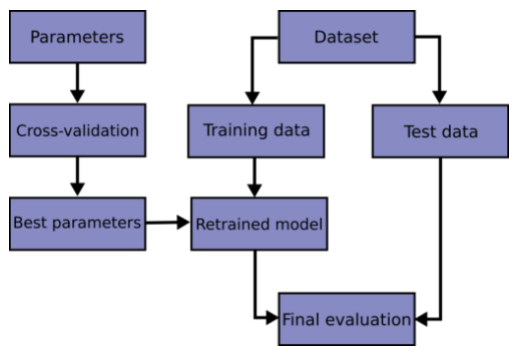
\includegraphics[width=7.5cm]{figures/process_graph.png} }
\caption{Cross-validation workflow in model training \cite{browne2000cross} } 
\label{fig}
\end{figure}

The validation data is taken from the training data, but is not involved in the training, so that the model can be evaluated relatively objectively on how well it matches the data outside the training set.

The evaluation of the model in the validation data is commonly done by cross-validation. It divides the original data into K-Folds, makes a separate validation set for each subset of data, and uses the remaining K-1 sets of subset data as the training set, which results in K models. These K models are evaluated separately in the validation set and the final error MSEs are summed and averaged to obtain the cross-validation error.

\begin{figure}[h]
\centering
\centerline{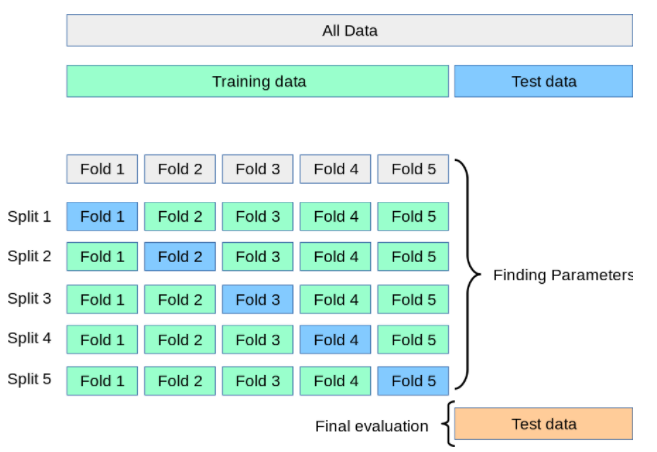
\includegraphics[width=8cm]{figures/cross_validation.png}}
\caption{K-fold cross-validation \cite{browne2000cross}}
\label{fig}
\end{figure}

In our project, we will set up a baseline ARIMA linear regression model, which is often used for time series forecasting. After that we will run different models, such as Support Vector Machines (SVM), Extra Trees, XGBoost, and AutoGluon, and compare the evaluation metrics of these models with the baseline. We will also compare different versions of our models after the cross-validation process and choose the best parameters. Then we compare the performance of different models and select the most appropriate algorithm for the final prediction task. From a technical standpoint, we believe that after parameter optimisation, it would be a huge improvement if the metrics of the best model represented an improvement of 10\% or more compared to the baseline.

\subsection{Data Exploration}

\textit{Figure 12} shows the correlations of variables in our data set with our main response variable, "MeanConsumption." We can see that the variables that seem most strongly positively correlated to mean consumption are hour and temperature. This makes sense: in terms of hour, lights tend to be off at night; people are sleeping so they consume fewer resources, and far fewer businesses operate at night. With regards to temperature, the use of AC systems and other cooling infrastructure is heavily determined by the outside temperature. On the other hand, humidity has the strongest negative correlation.


\begin{figure}[h]
\centering
\centerline{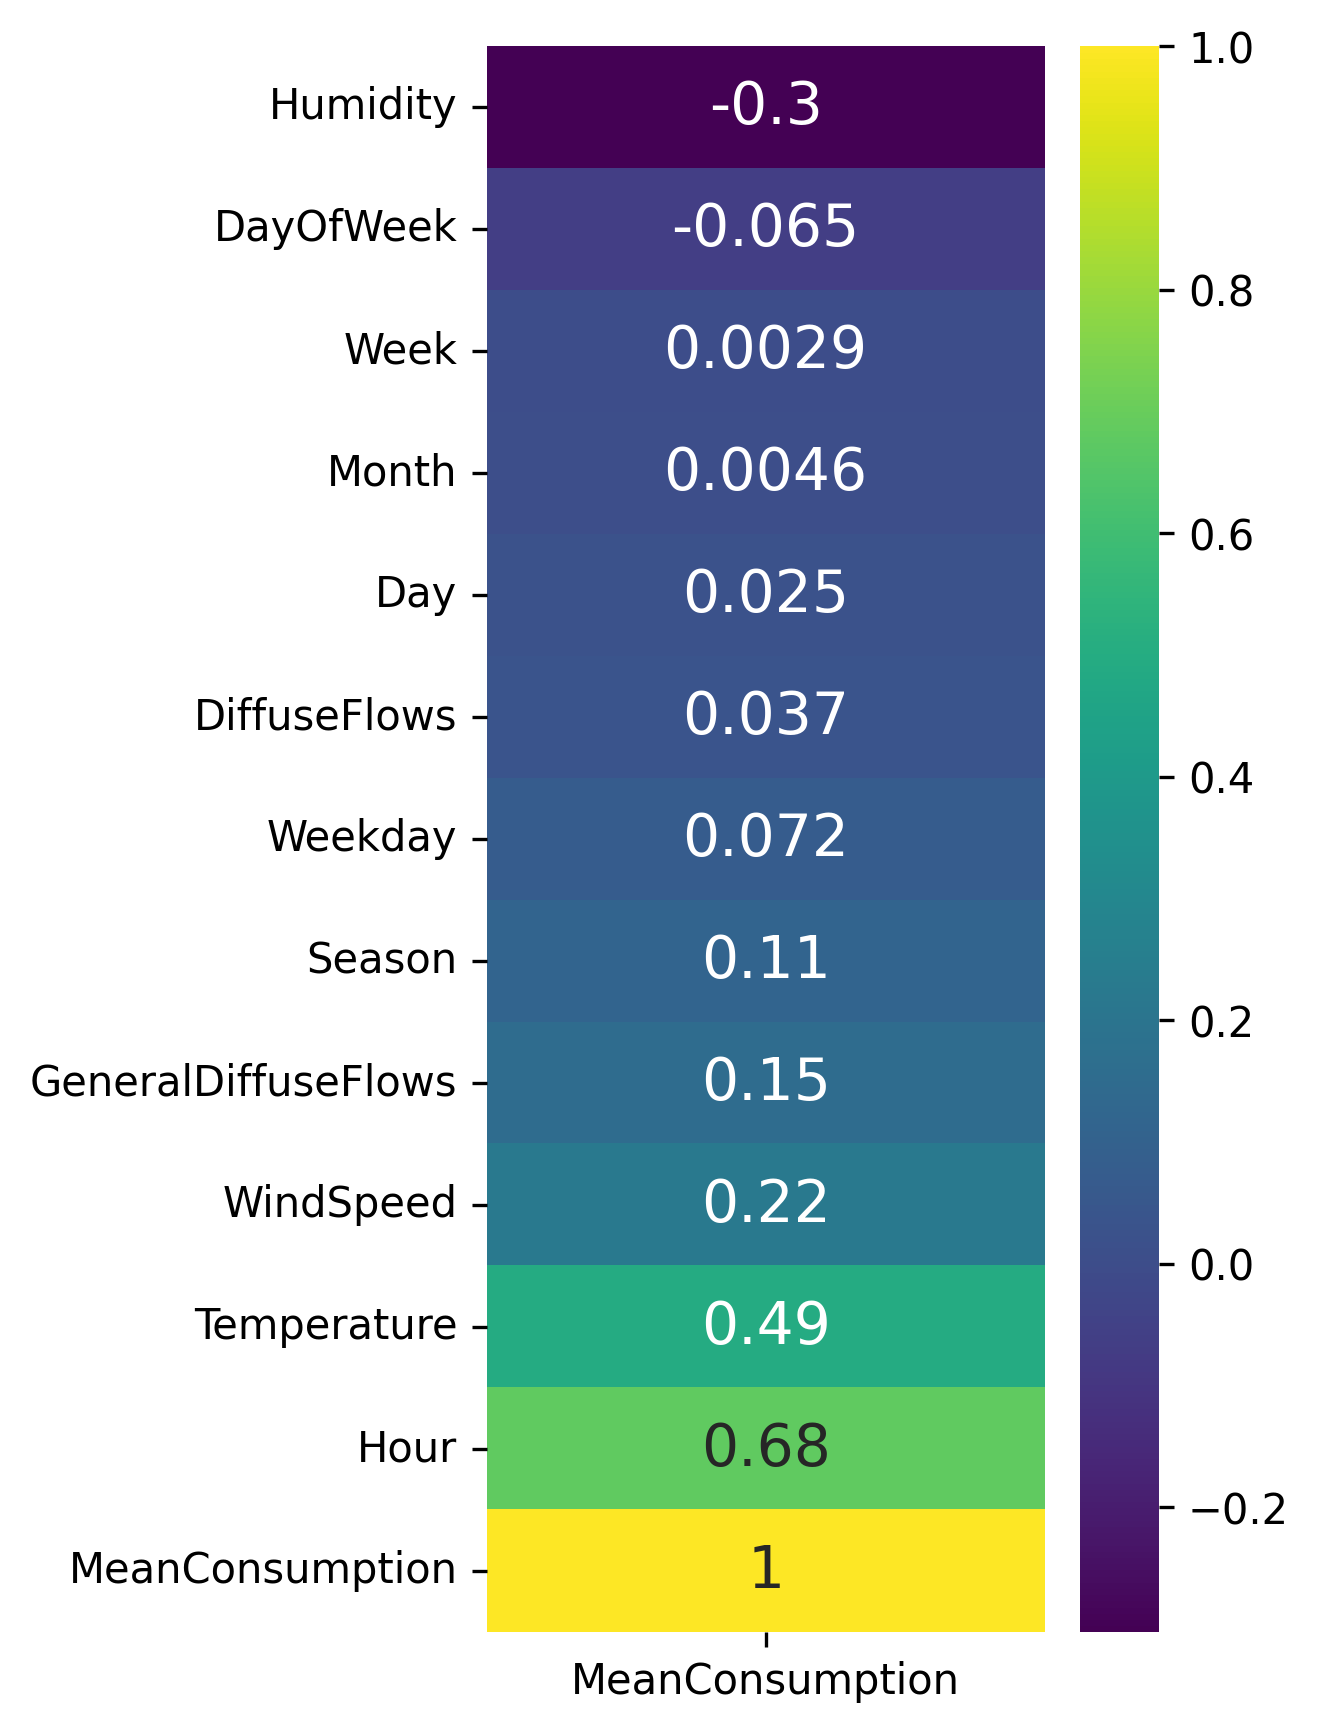
\includegraphics[width=5cm]{figures/corrmat-2.png}}
\caption{Correlation matrix for the power consumption of the city of Tetouan.}
\label{fig}
\end{figure}


\subsection{Remainder of the Forecast Plots from the Baseline model}
The plots in this section provide information on both the naive and composite forecasts of the ARIMA model across forecast horizon.
\begin{figure}[h]
\centering
\centerline{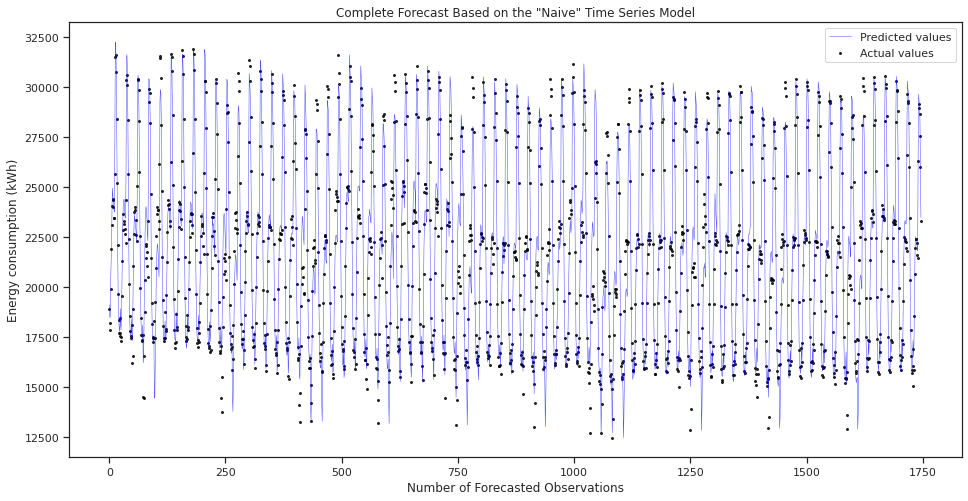
\includegraphics[width=8cm]{figures/Naive_forecast.png}}
\caption{Naive forecast across forecast horizon}
\label{fig_naiveplot}
\end{figure}

\begin{figure}[h]
\centering
\centerline{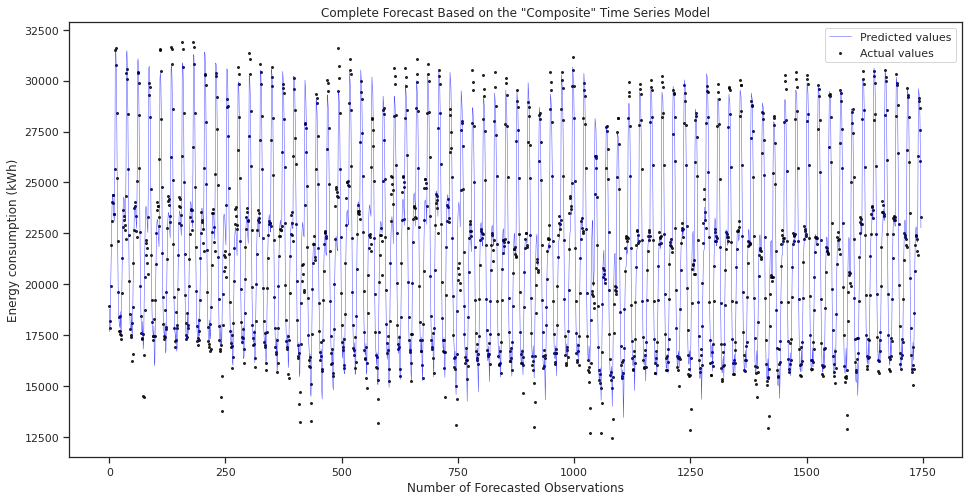
\includegraphics[width=8cm]{figures/Composite_forecast.png}}
\caption{Composite forecast across forecast horizon}
\label{fig_compplot}
\end{figure}

\subsection{Stationary Time Series}
We provide in this section a plot of the stationary time-series obtained by calculating 1-hour differences of the Mean Consumption values. 
\begin{figure}[h]
\centering
\centerline{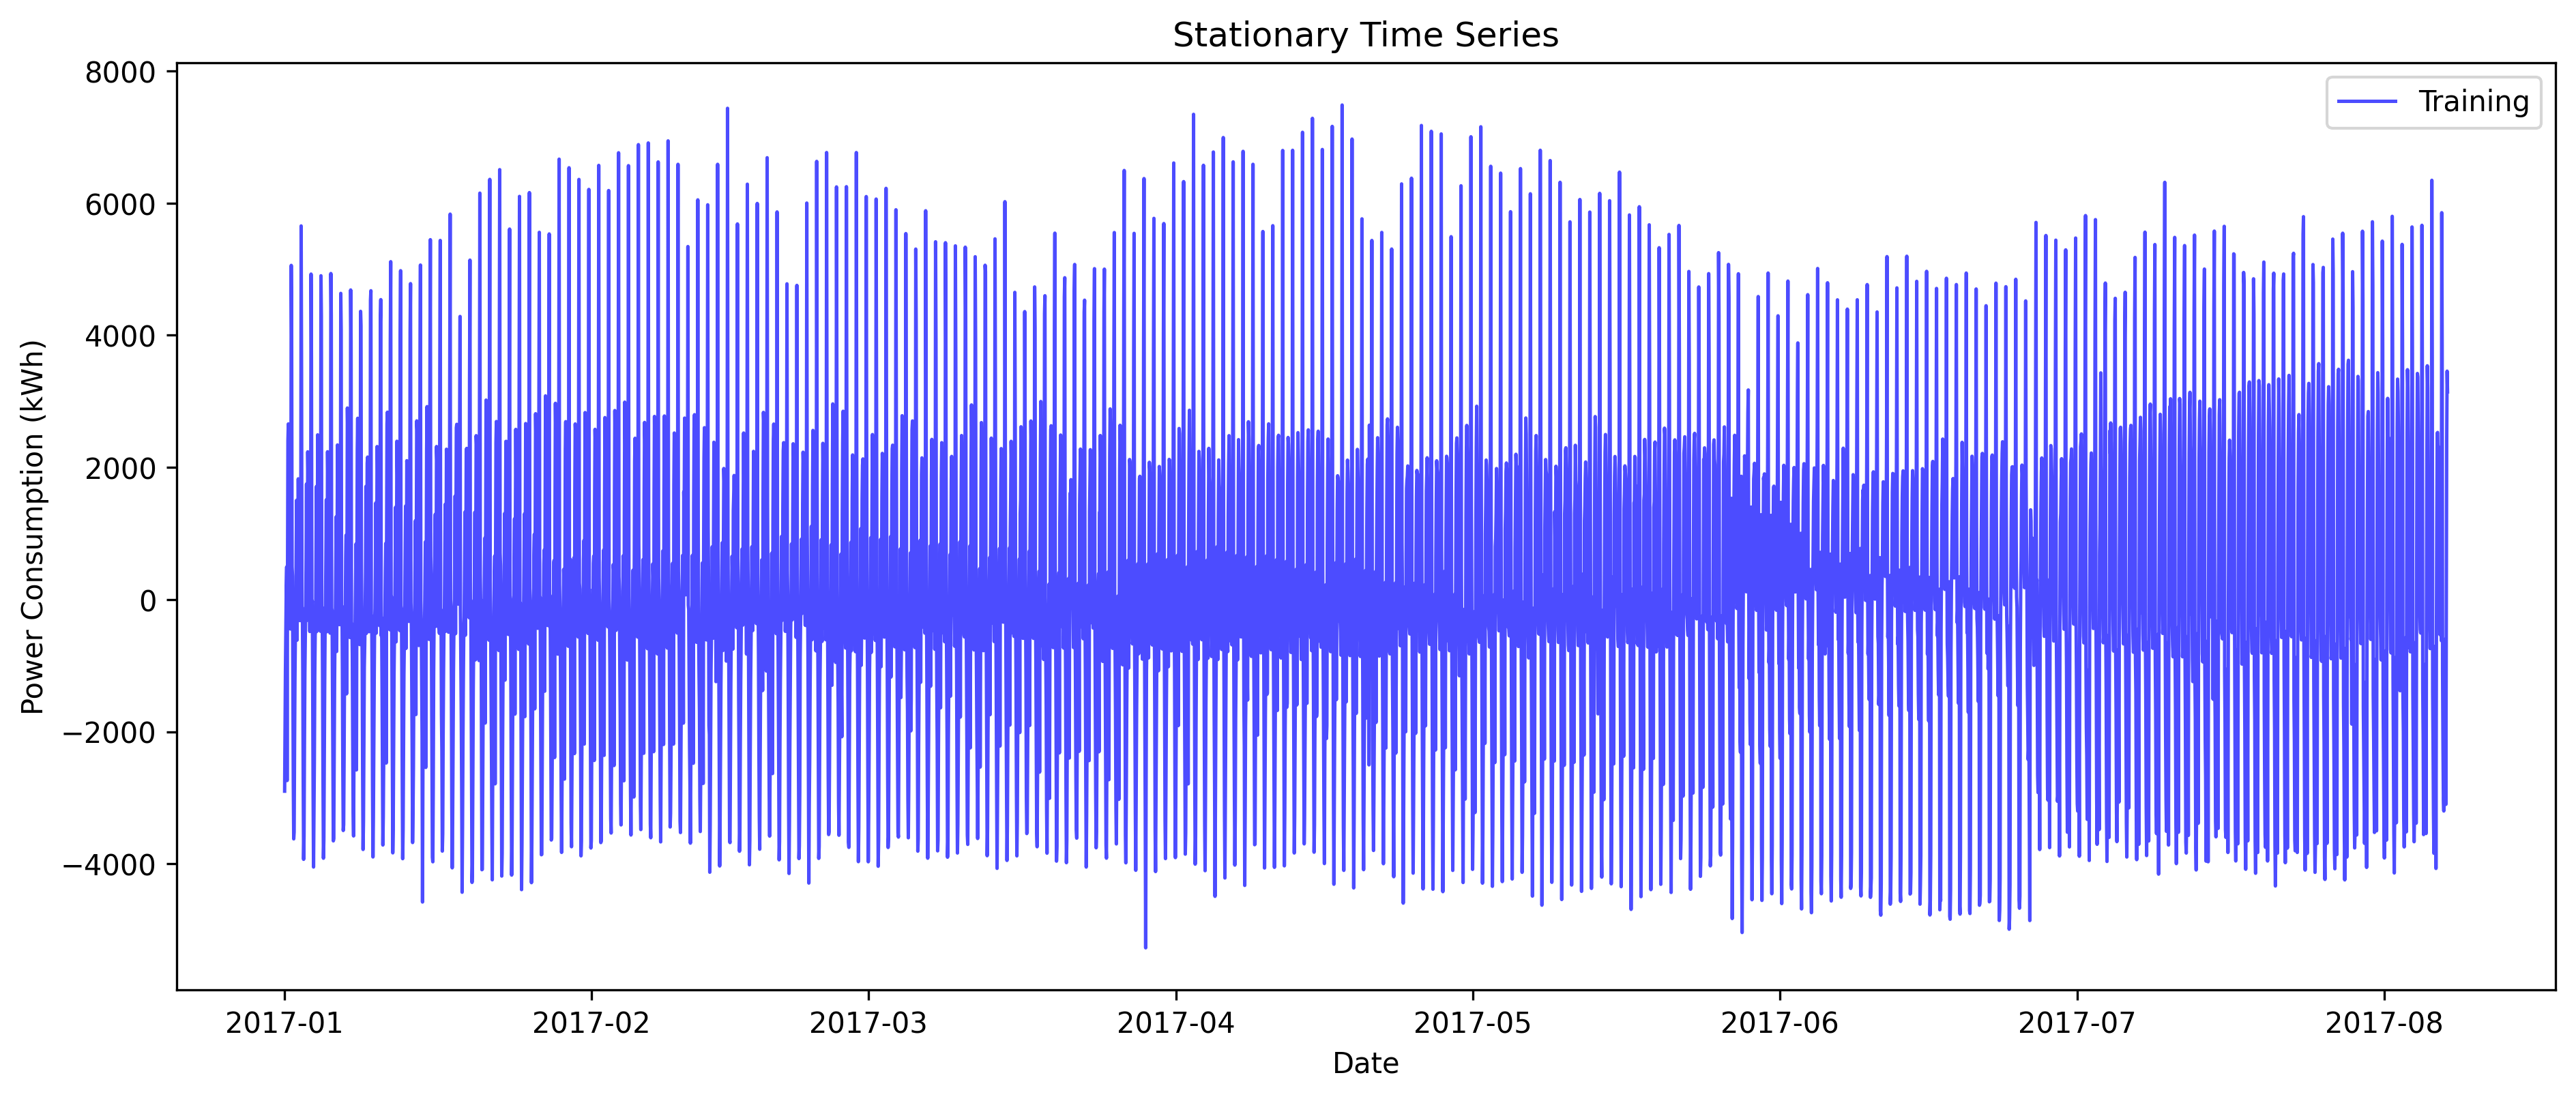
\includegraphics[width=8cm]{figures/StationaryTS.png}}
\caption{Time series after differencing mean consumption values}
\label{fig_stationary}
\end{figure}

\end{document}
